\documentclass[12pt,UTF8,fleqn]{ctexart}
\usepackage{ctex,amsmath,amssymb,geometry,fancyhdr,bm,amsfonts,mathtools,extarrows,graphicx,url,enumerate,xcolor,float,multicol,wasysym}
\usepackage{subfigure}
\allowdisplaybreaks[4]
% 加入中文支持
\newcommand\Set[2]{\left\{#1\ \middle\vert\ #2 \right\}}
\newcommand\Lim[0]{\lim\limits_{n\rightarrow\infty}}
\newcommand\LIM[2]{\lim\limits_{#1\rightarrow#2}}
\newcommand\Ser[1]{\sum_{n=#1}^\infty}
\newcommand{\SER}[2]{\sum_{#1=#2}^\infty}
\newcommand{\Int}[4]{\varint\nolimits_{#1}^{#2}#3\mathrm d#4}
\newcommand{\aIInt}[1]{\iint\limits_{#1}}
\newcommand{\IInt}[3]{\iint\limits_{#1}#2\mathrm d#3}
\newcommand{\varIInt}[4]{\iint\limits_{#1}#2\mathrm d#3\mathrm d#4}
\newcommand{\IIInt}[3]{\iiint\limits_{#1}#2\mathrm d#3}
\newcommand{\varIIInt}[5]{\iiint\limits_{#1}#2\mathrm d#3\mathrm d#4\mathrm d#5}
\newcommand{\LInt}[3]{\varint\nolimits_{#1}#2\mathrm d#3}
\newcommand{\LOInt}[3]{\varoint\nolimits_{#1}#2\mathrm d#3}
\newcommand{\LLInt}[4]{\varint\nolimits_{#1}\nolimits^{#2}#3\mathrm d#4}
\newcommand{\BLInt}[2]{\varint\nolimits_{#1}#2}
\newcommand{\varBLInt}[3]{\varint\nolimits_{#1}\nolimits^{#2}#3}
\newcommand{\BLOInt}[2]{\varoint\nolimits_{#1}#2}
\newcommand{\SIInt}[3]{\iint\limits_{#1}#2\mathrm d#3}
\newcommand{\md}[1]{\mathrm d#1}
\newcommand{\BSIInt}[2]{\iint\limits_{#1}#2}
\newcommand{\pp}[2]{\frac{\partial #1}{\partial #2}}
\newcommand{\ppx}[1]{\frac{\partial #1}{\partial x}}
\newcommand{\ppy}[1]{\frac{\partial #1}{\partial y}}
\newcommand{\ppz}[1]{\frac{\partial #1}{\partial z}}
\newcommand{\varppx}[1]{\frac{\partial}{\partial x} #1}
\newcommand{\varppy}[1]{\frac{\partial}{\partial y} #1}
\newcommand{\varppz}[1]{\frac{\partial}{\partial z} #1}
\newcommand{\BSOIInt}[2]{\oiint\limits_{#1}#2}
\newcommand{\me}[0]{\mathrm e}
\geometry{a4paper,scale=0.80}
\pagestyle{fancy}
\rhead{向量场的微积分(5)}
\lhead{基础习题课期末复习}
\chead{微积分B(2)}
\begin{document}
\setcounter{section}{13}
\section{保守场、向量场的微分运算}
\subsection{复习计划}
\begin{figure}[H]
\begin{center}
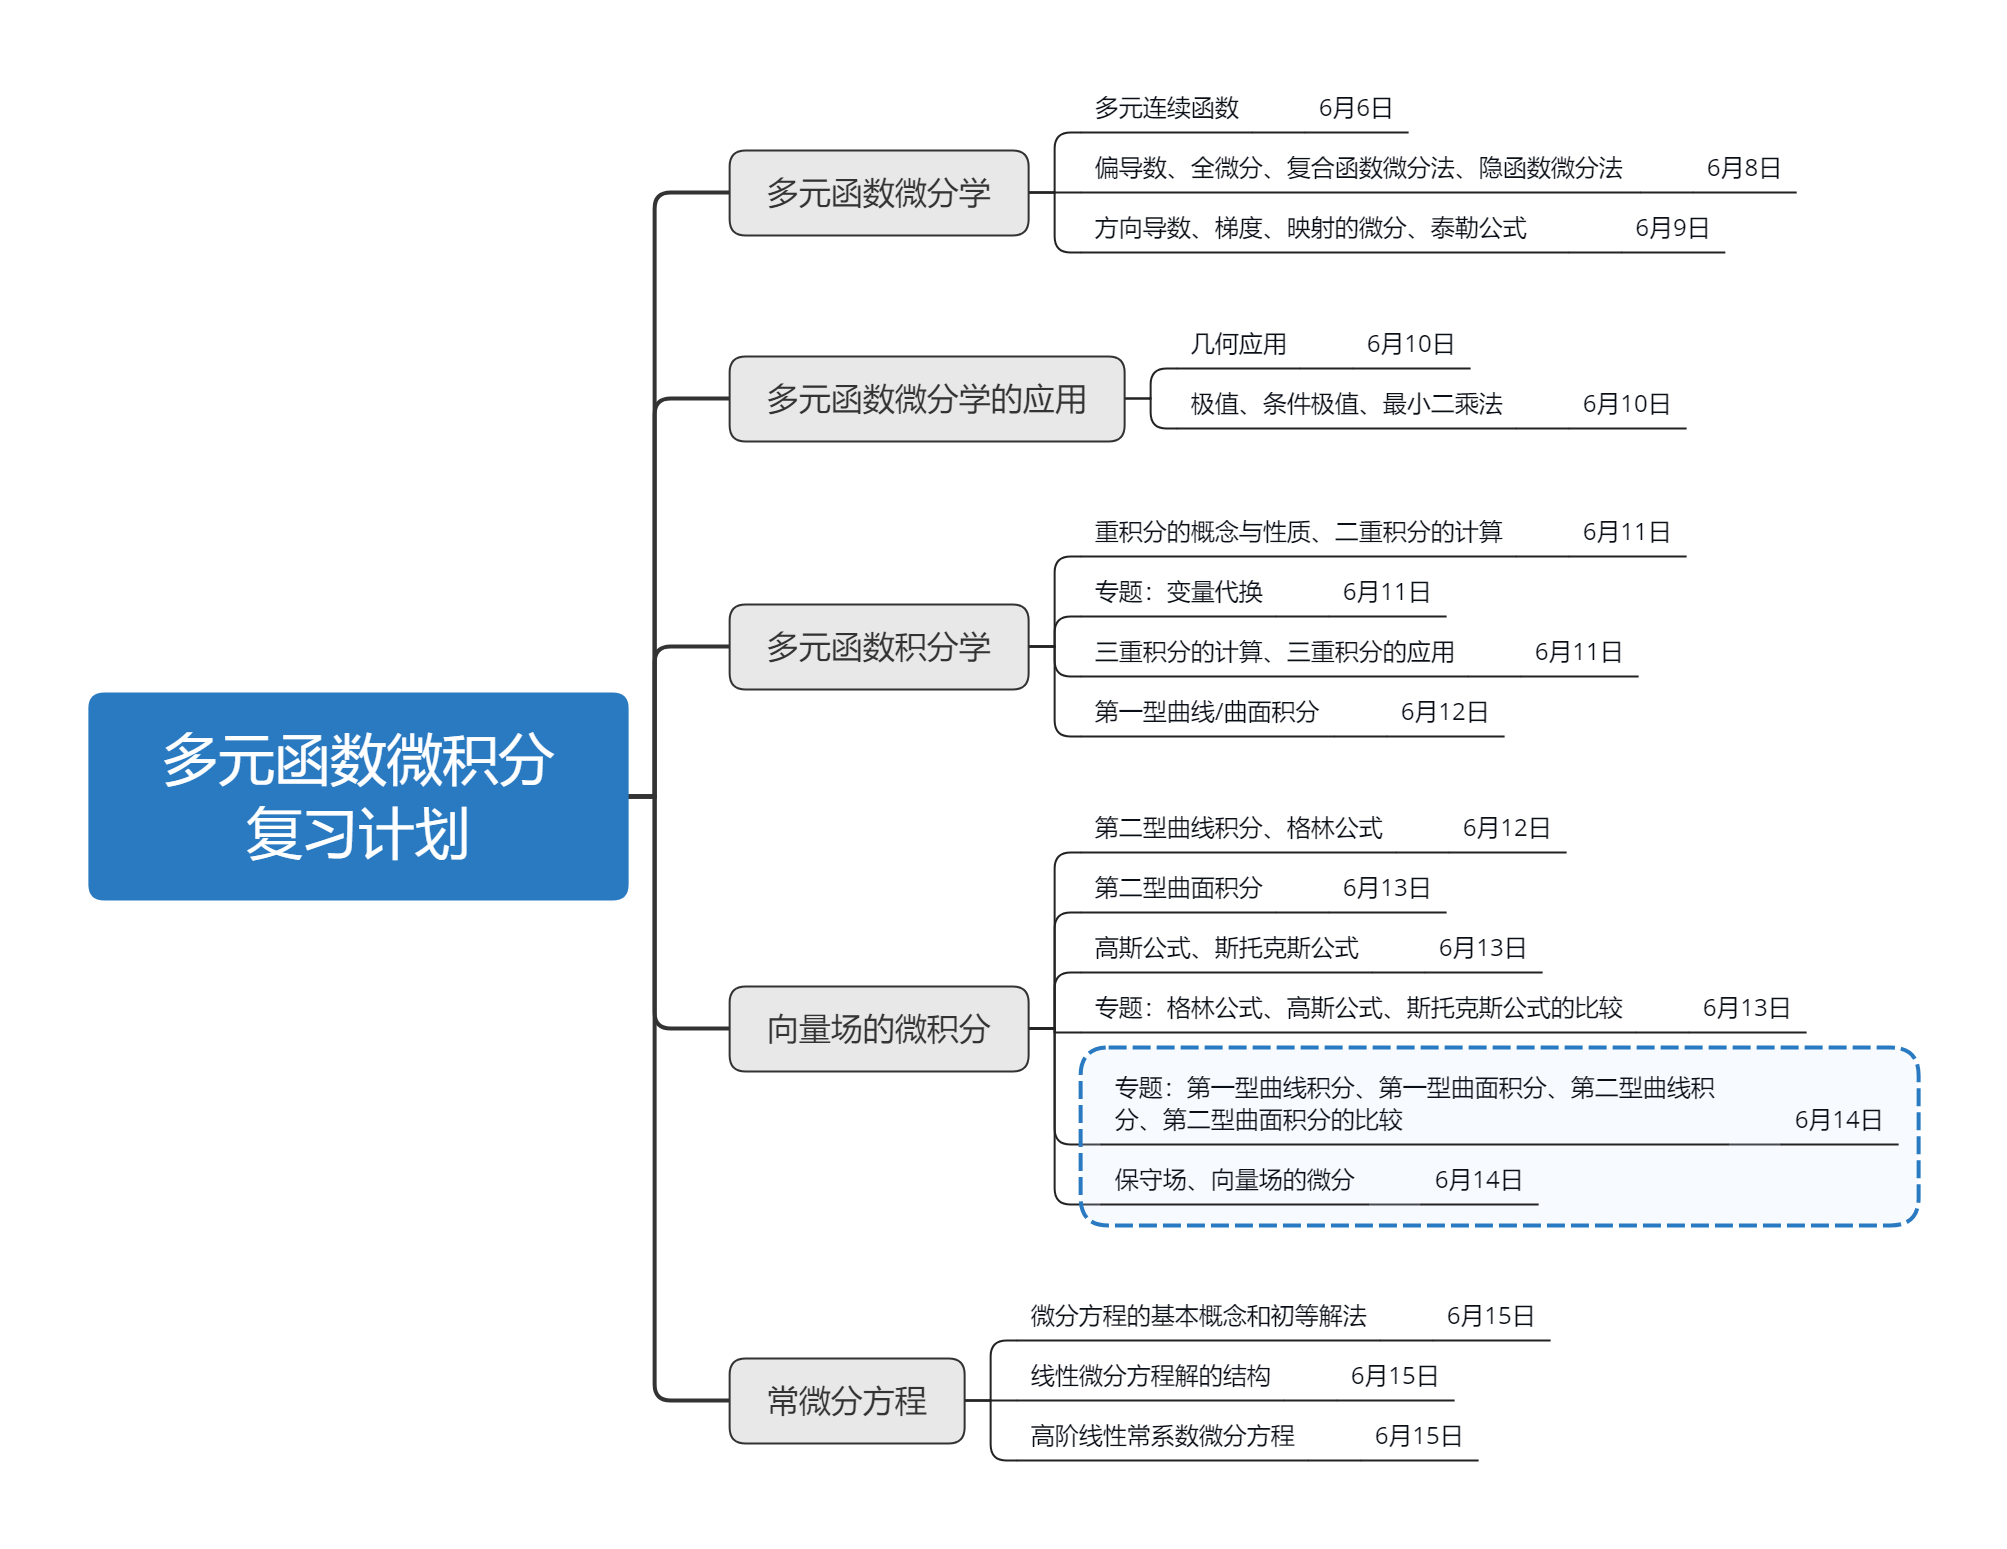
\includegraphics[height=0.5\textheight]{Figures20190614/plan.png}
\end{center}
\end{figure}
\subsection{知识结构}
\begin{figure}[H]
\begin{center}
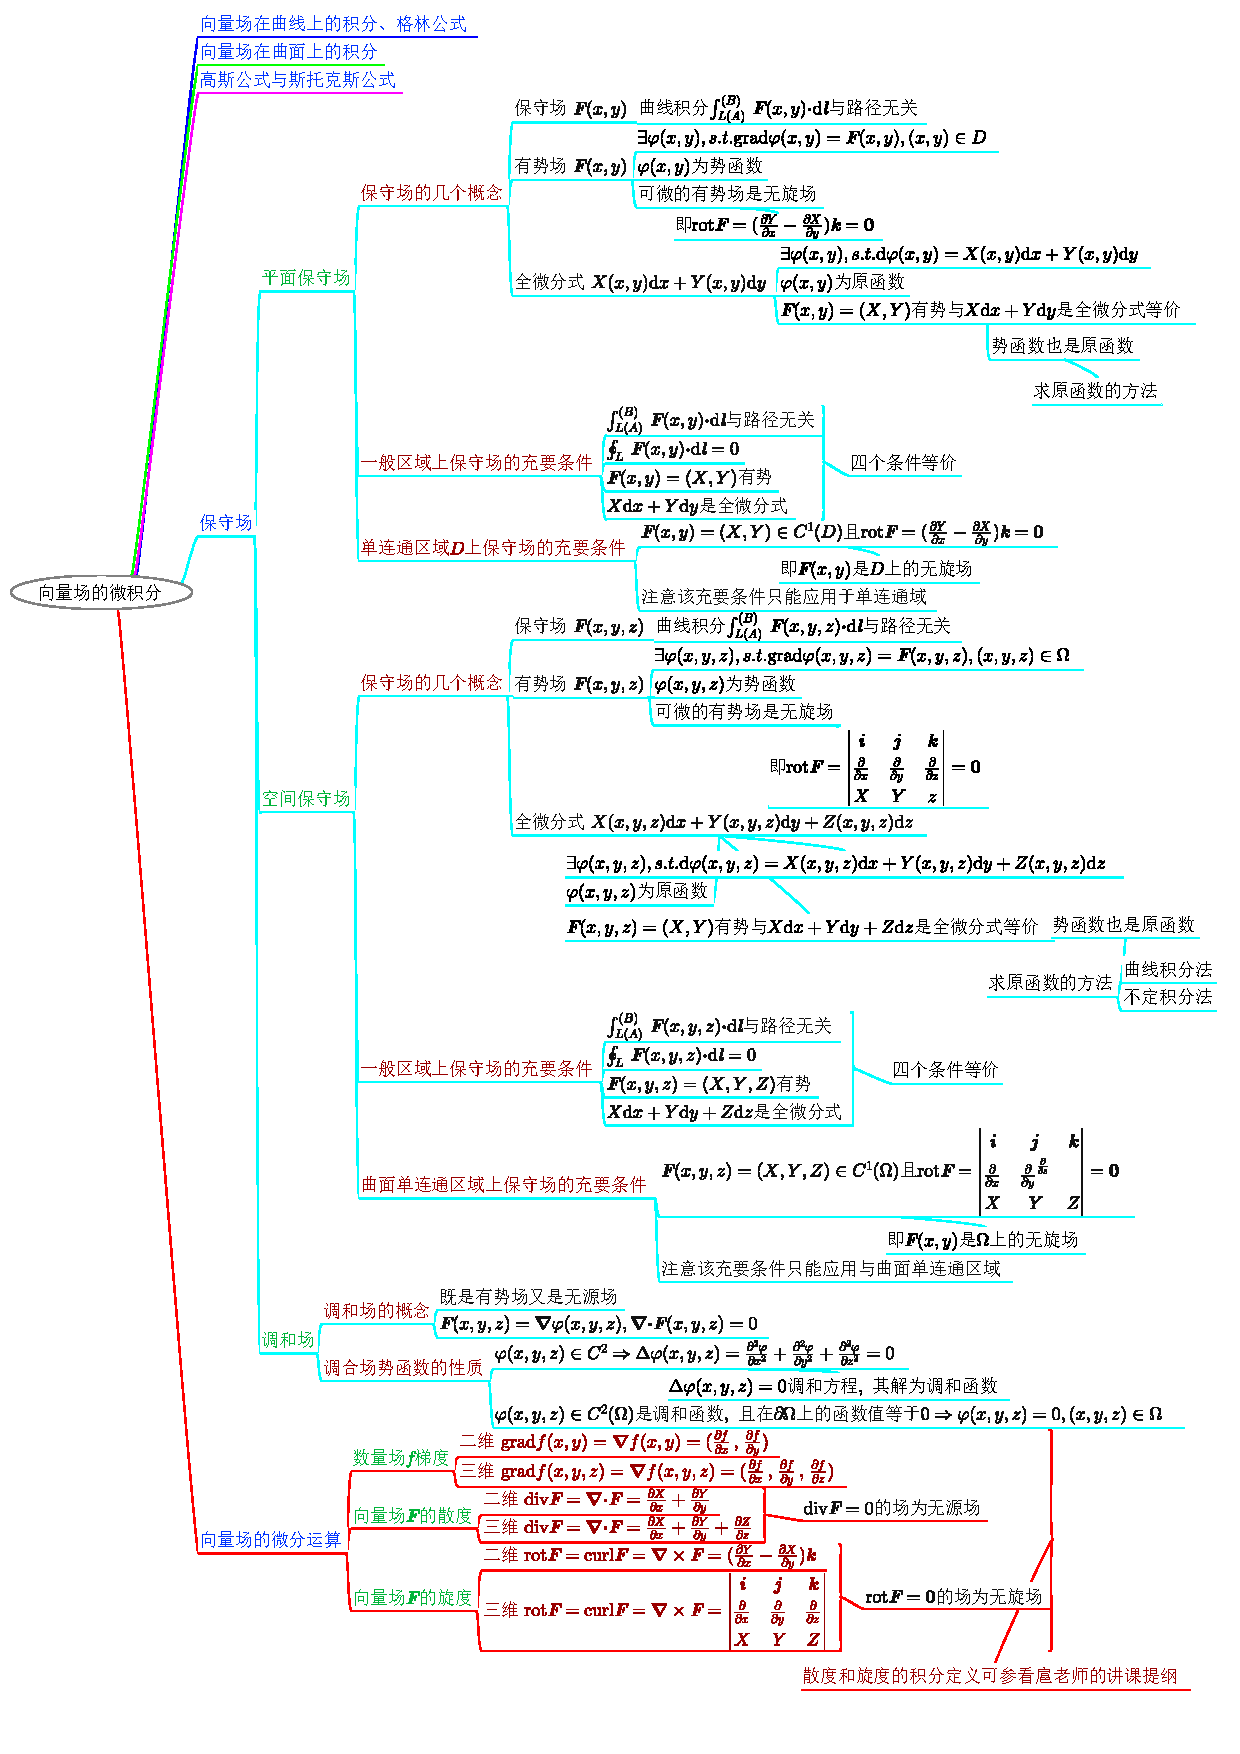
\includegraphics[height=1\textheight]{20190614.pdf}
\end{center}
\end{figure}
\subsection{保守场}

平面保守场的性质如下所示。

\begin{figure}[H]
\begin{center}
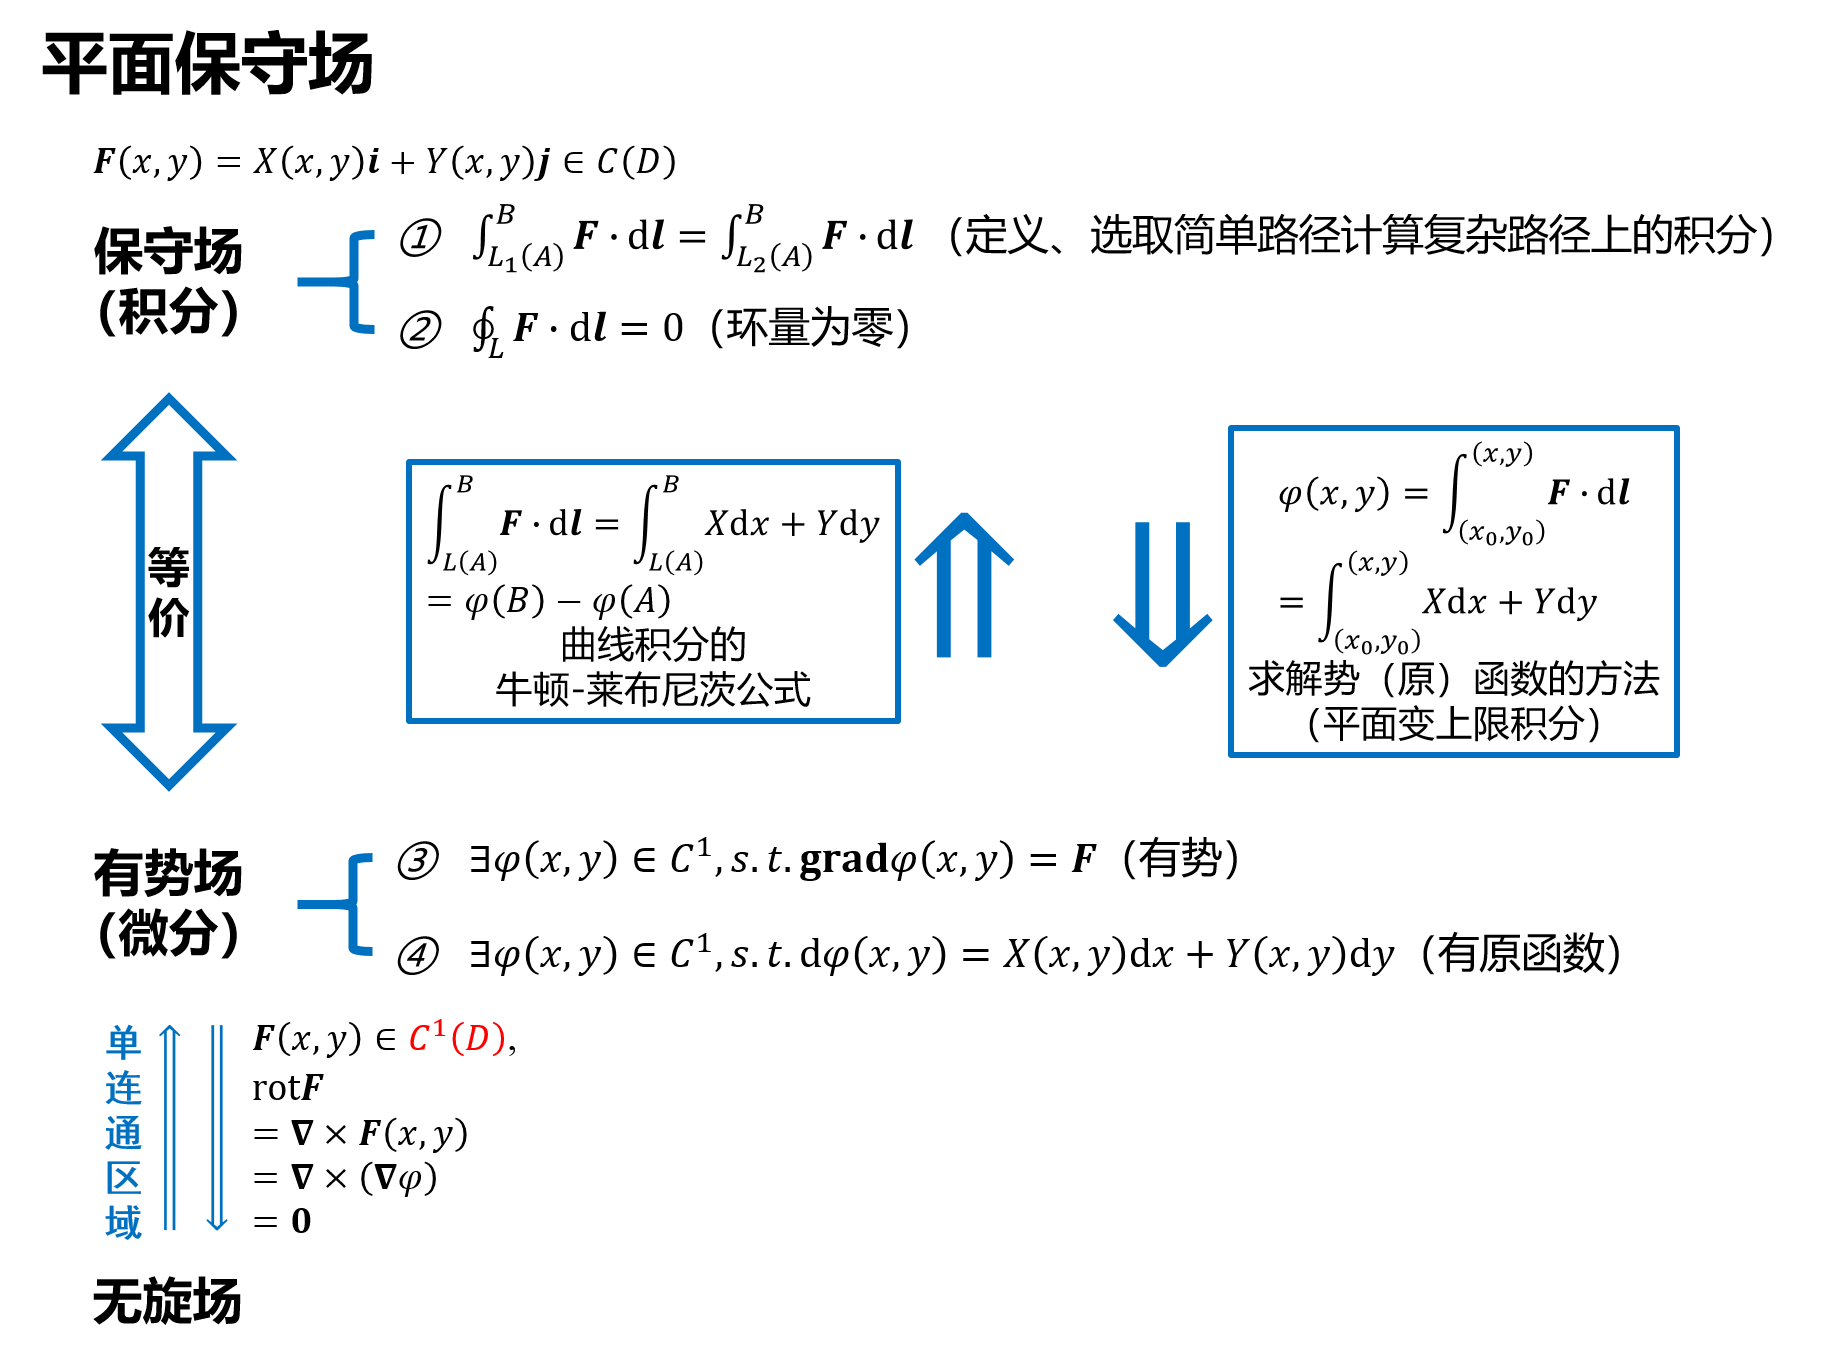
\includegraphics[height=0.54\textheight]{Figures25/PlaneConserv.png}
\end{center}
\end{figure}

\noindent{\bf说明:}
\begin{enumerate}
\item性质\textcircled{1}中的简单路径可选为与坐标轴平行的直线或折线路径. 

\begin{figure}[H]
\begin{center}
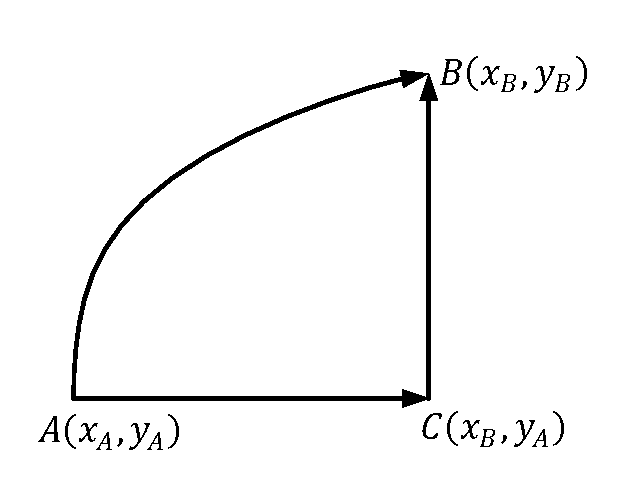
\includegraphics[height=0.25\textheight]{Figures25/Fig13-6-Intro-2.pdf}
\end{center}
\caption{与坐标轴平行的折线路径.}
\label{13-6-Intro}
\end{figure}

在与$x$轴平行的直线路径$AC$上,积分$\varint_{L(A)}^C{\bm F\bm\cdot\md\bm l}=\varint_{L(A)}^C{X(x,y)\md x+Y(x,y)\md y}$的被积表达式$X(x,y)\md x+Y(x,y)\md y$中$\md y=0,y=y_A$,故
\[\varint\nolimits_{L(A)}\nolimits^C{\bm F\bm\cdot\md\bm l}=\varint\nolimits_{(x_A,y_A)}\nolimits^{(x_B,y_A)}{X(x,y)\md x+Y(x,y)\md y}=\Int{x_A}{x_B}{X(x,y_A)}x.\]
在与$y$轴平行的直线路径$CB$上,积分$\varint_{L(C)}^B{\bm F\bm\cdot\md\bm l}=\varint_{L(C)}^B{X(x,y)\md x+Y(x,y)\md y}$的被积表达式$X(x,y)\md x+Y(x,y)\md y$中$\md x=0,x=x_B$,故
\[\varint\nolimits_{L(C)}\nolimits^B{\bm F\bm\cdot\md\bm l}=\varint\nolimits_{(x_B,y_A)}\nolimits^{(x_B,y_B)}{X(x,y)\md x+Y(x,y)\md y}=\Int{y_A}{y_B}{Y(x_B,y)}y.\]
【考察这一点的习题:1.(1)/(2)/(3)/(4),3.(1)/(2). (第一类题目)】
%\begin{figure}[H]
%\centering 
%\subfigure[] { \label{13-6-Intro-1} 
%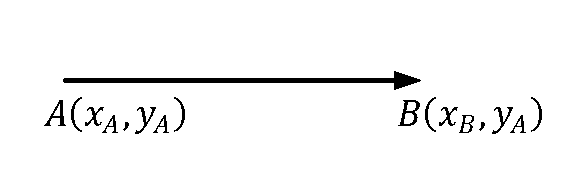
\includegraphics[height=0.1\textheight]{Figures25/Fig13-6-Intro-1.pdf} } 
%\subfigure[] { \label{13-6-Intro-2} 
%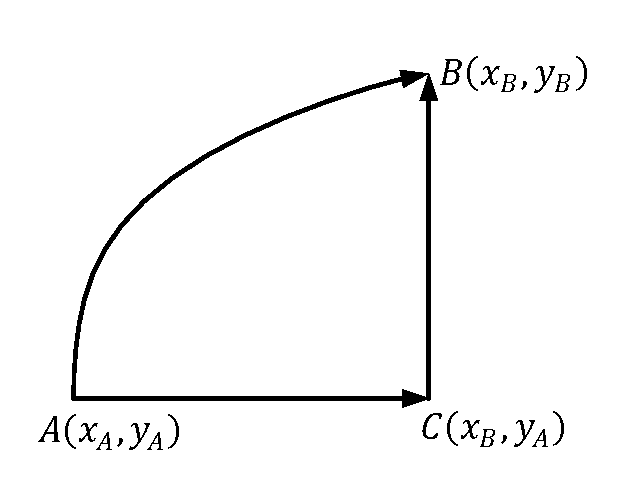
\includegraphics[height=0.3\textheight]{Figures25/Fig13-6-Intro-2.pdf} } 
%\caption{与坐标轴平行的直线或折线路径.} 
%\label{13-6-Intro} 
%\end{figure} 
\item\textcircled{1},\textcircled{2},\textcircled{3},\textcircled{4}相互等价,既是性质定理也是判定定理,知道其中一个即可判定该向量场是保守场,也就可以得到另外三个性质.
\item保守场是有势场,有势场也是保守场,二者是完全等价的概念. 保守场的两个性质从积分角度描述了向量场,有势场的两个性质从微分角度描述了向量场.
\item可通过对势函数这样一个数量场的分析来对向量场进行分析,比如可以用引力势能分析引力场,用重力势能分析重力场,用电势能分析电场力的场,用电势分析电场。
\item势函数与原函数相同.
\item可微的保守场是无旋场(但无旋场不一定是保守场). 

【考察这一点的习题:2. (第二类题目)】
\item平面单连通域上的无旋场是保守场. 常利用平面单连通区域上无旋来判定一个向量场是保守场.

【考察这一点的习题:1.(1)/(2)/(3)/(4),3.(1)/(2). (第一类题目)】

\item可微场才可用旋度算子计算旋度. 如一个向量场不可微,则不可用旋度算子计算旋度,难以用旋度为零来判断该向量场是保守场.

【考察这一点的习题:4. (第三类题目)】

\item求解全微分式的原函数有两种方法,变上限积分法和不定积分法.

【考察这一点的习题:3.(1)/(2). (第四类题目)】
\item空间保守场的性质与平面保守场类似,主要的不同是三维空间中的曲面单连通域(比如球壳是曲面单连通域,圆环体则不是曲面单连通域)上的无旋场是保守场。
\end{enumerate}
\subsection{无源场、无旋场}
\begin{enumerate}
\item无源场$\text{div}\bm F=\bm\nabla\bm\cdot\bm F=0$.

【与无源场有关的题目:5,7,8.(1)/(2),9. (第五类题目)】

\item无旋场$\text{rot}\bm F=\bm\nabla\times\bm F=\bm0$.

【与无旋场有关的题目:6,10.(1)/(2). (第六类题目)】

【综合题目:9. (主要考察通量的概念、高斯公式、无源场)】
\end{enumerate}
\subsection{向量场的微分运算习题分类}
\begin{enumerate}
\item验证三个算子的性质.

【习题13.1中的1., 2., 4.】

\item求梯度、散度、旋度.

【习题13.1中的3., 5., 6.】
\end{enumerate}
\subsection{习题13.6解答}
\begin{enumerate}
\item利用积分域与路线无关的性质计算下列积分:\\
(1)$\BLInt L{(x^3+xy^2)\md x+(y^3+x^2y)\md y}$,其中$L$为从$O(0,0)$经$A(1,1)$到$B(2,0)$的折线;\\
(2)$\BLInt L{(y+1)\tan x\md x-\ln\cos x\md y}$,其中$L$为曲线$x=\cos t,y=2\sin t(0\leqslant t\leqslant\pi)$,顺时针方向;\\
(3)$\BLInt L{(\ln\frac yx-1)\md x+\frac xy\md y}$,其中$L$为由点$A(1,1)$出发到$B(\me,3\me)$的任何一条不与$x$轴以及$y$轴相交的曲线;\\
(4)$\BLInt L{\frac{1+y^2f(xy)}y\md x+\frac x{y^2}[y^2f(xy)-1]\md y}$,其中$L$为由点$A(0,1)$出发到$B(1,2)$的任何一条不与$x$轴相交的曲线,$f$是连续可微的函数.

解:(1)\begin{figure}[H]
\begin{center}
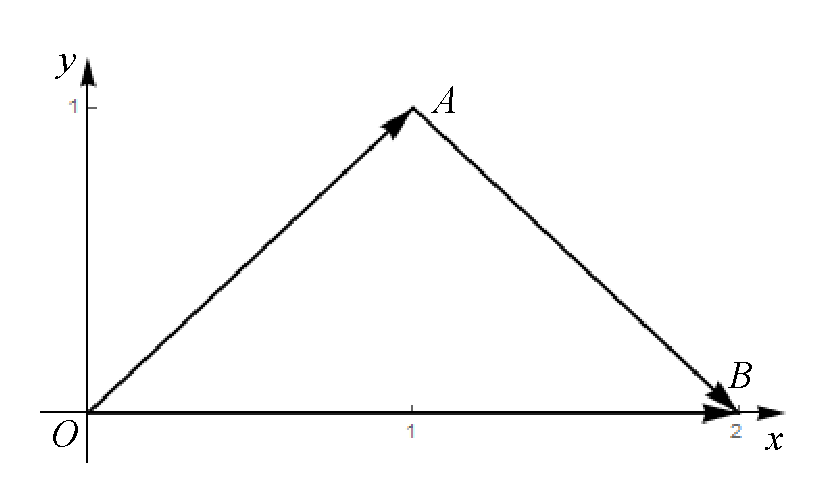
\includegraphics[height=0.2\textheight]{Figures25/Fig13-6-1-1.pdf}
\end{center}
\caption{习题13.6 1.(1)题图示}
\label{13-6-1-1}
\end{figure}

令$\begin{cases}
X(x,y)=x^3+xy^2,\\
Y(x,y)=y^3+x^2y,
\end{cases}$则$\bm F(x,y)=(X,Y)\in C^1(\mathbb R)$, 

$\because\mathbb R$为单连通域,

且$\text{rot}\bm F=(\pp Yx-\pp Xy)\bm k=(2xy-2xy)\bm k=\bm0$,

$\therefore\BLInt L{X\md x+Y\md y}=\varint_{(0,0)}^{(2,0)}{X\md x+Y\md y}=\Int02{x^3}x=\frac14x^4\big|_0^2=4$.

(2)\begin{figure}[H]
\begin{center}
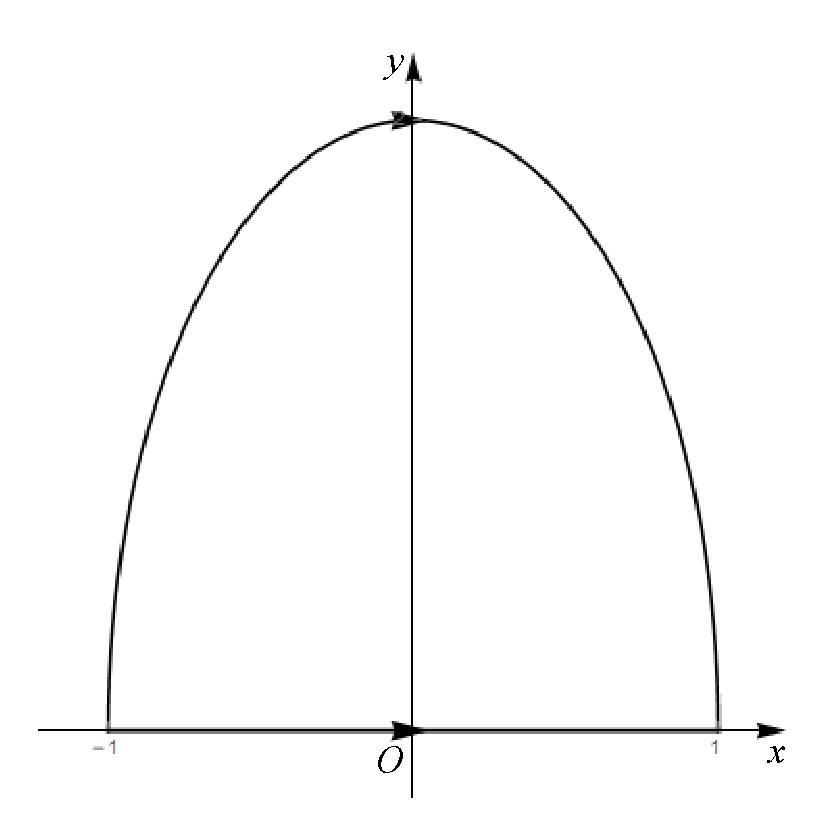
\includegraphics[height=0.3\textheight]{Figures25/Fig13-6-1-2.pdf}
\end{center}
\caption{习题13.6 1.(2)题图示}
\label{13-6-1-2}
\end{figure}

曲线$L:\begin{cases}
x=\cos t,\\
y=2\sin t,
\end{cases}(0\leqslant t\leqslant\pi)$为一椭圆弧$x^2+\frac{y^2}4=1,y\geqslant0$,顺时针的起点为$(-1,0)$终点为$(1,0)$,

设$D=(-\frac\pi2,\frac\pi2)\times(-\infty,\infty)$,则$L\in D$,

令$\begin{cases}
X(x,y)=(y+1)\tan x,\\
Y(x,y)=-\ln\cos x,
\end{cases}$则$\bm F(x,y)=(X,Y)\in C^1(D)$,

$\because D$是单连通区域,

且$\text{rot}\bm F=(\pp Yx-\pp Xy)\bm k=(-\frac{-\sin x}{\cos x}-\tan x)\bm k=\bm0$,

$\therefore\BLInt L{X\md x+Y\md y}=\varint_{(-1,0)}^{(1,0)}{X\md x+Y\md y}=\Int{-1}1{\tan x}x=0$.

(3)
\begin{figure}[H]
\begin{center}
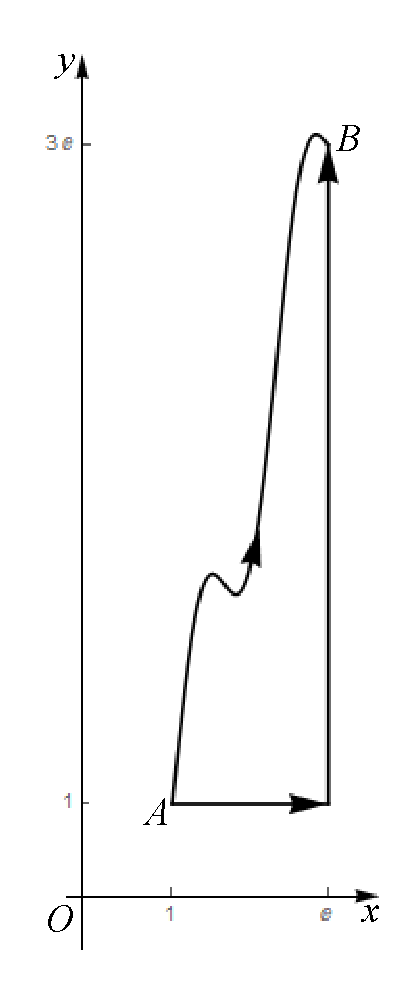
\includegraphics[height=0.5\textheight]{Figures25/Fig13-6-1-3.pdf}
\end{center}
\caption{习题13.6 1.(3)题图示}
\label{13-6-1-3}
\end{figure}

设$D=\Set{(x,y)}{x>0,y>0}$,则$L\in D$,

令$\begin{cases}
X(x,y)=\ln\frac yx-1,\\
Y(x,y)=\frac xy,
\end{cases}$则$\bm F(x,y)=(X,Y)\in C^1(D)$,

$\because D$是单连通域,

且$\text{rot}\bm F=(\pp Yx-\pp Xy)\bm k=(\frac1y-\frac1{\frac yx}\frac1x)\bm k=\bm0$,

$\therefore\BLInt L{X\md x+Y\md y}=\varint_{(1,1)}^{(\me,3\me)}{X\md x+Y\md y}=\varint_{(1,1)}^{(\me,1)}{X\md x+Y\md y}+\varint_{(\me,1)}^{(\me,3\me)}{X\md x+Y\md y}\\
=\Int1\me{(\ln\frac1x-1)}x+\Int1{3\me}{\frac\me y}y=x(-\ln x-1)\big|_1^\me-\Int1\me x{(-\ln x-1)}+\me\ln y\big|_1^{3\me}\\
=\me(-1-1)-1\cdot(0-1)+\Int1\me{x\frac1x}x+\me\ln{3\me}-0=-2\me+1+(\me-1)+\me\ln3+\me=\me\ln3$.

(4)
\begin{figure}[H]
\begin{center}
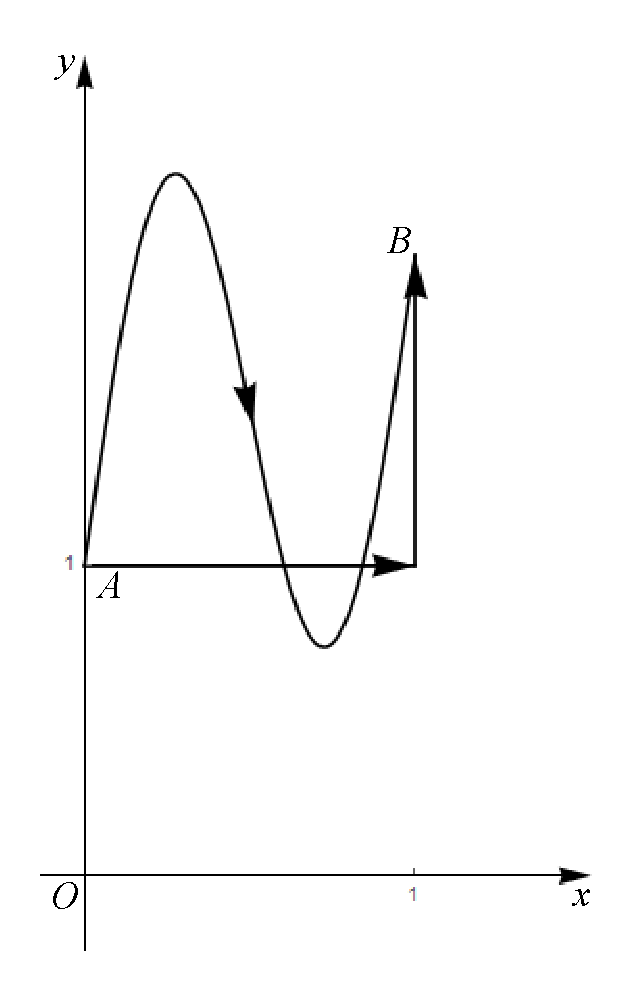
\includegraphics[height=0.5\textheight]{Figures25/Fig13-6-1-4.pdf}
\end{center}
\caption{习题13.6 1.(4)题图示}
\label{13-6-1-4}
\end{figure}

设$D=\Set{(x,y)}{y>0}$,

令$\begin{cases}
X(x,y)=\frac{1+y^2f(xy)}y=\frac1y+yf(xy),\\
Y(x,y)=\frac x{y^2}[y^2f(xy)-1]=xf(xy)-\frac x{y^2},
\end{cases}$则$\bm F(x,y)=(X,Y)\in C^1(D)$,

$\because D$单连通,

且$\text{rot}\bm F=(\pp Yx-\pp Xy)\bm k=\{f(xy)+xf'(xy)y-\frac1{y^2}-[-\frac1{y^2}+f(xy)+yf'(xy)x]\}\bm k=\bm0$,

$\therefore\BLInt L{X\md x+Y\md y}=\varint_{(0,1)}^{(1,2)}{X\md x+Y\md y}=\varint_{(0,1)}^{(1,1)}{X\md x+Y\md y}+\varint_{(1,1)}^{(1,2)}{X\md x+Y\md y}\\
=\Int01{[1+f(x)]}x+\Int12{[f(y)-\frac1{y^2}]}y=\Int01{}x+\Int01{f(x)}x+\Int12{f(y)}y-\Int12{\frac1{y^2}}y\\
=1+\Int02{f(x)}x+\frac1y\big|_1^2=\frac12+\Int02{f(x)}x$.

\item确定$p$的值,使积分$\varint_A^B{(x^4+4xy^p)\md x+(6x^{p-1}y^2-5y^4)\md y}$与路线无关. 当$A=(0,0),B=(1,2)$时,计算积分的值.

\begin{figure}[H]
\begin{center}
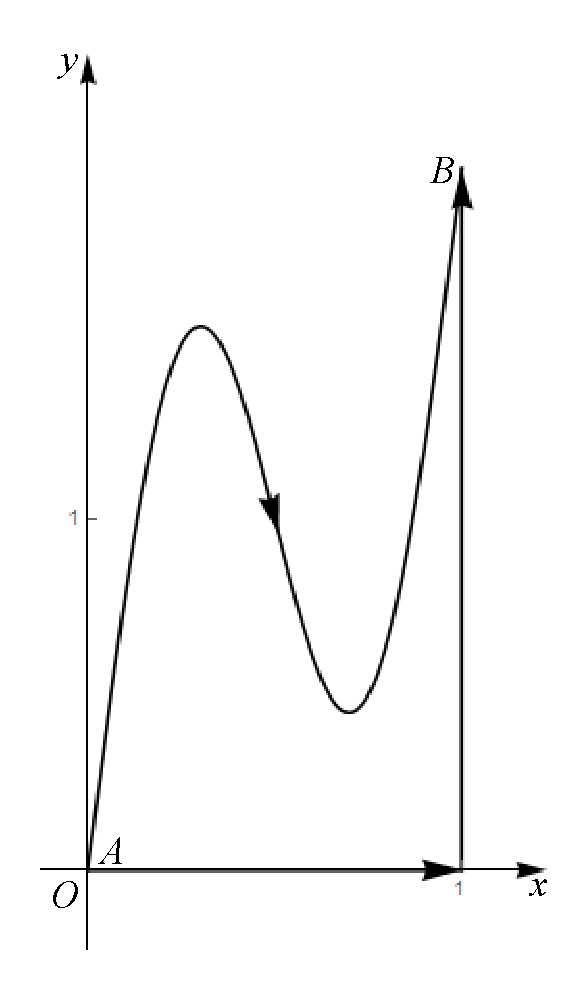
\includegraphics[height=0.5\textheight]{Figures25/Fig13-6-2.pdf}
\end{center}
\caption{习题13.6 2.题图示}
\label{13-6-2}
\end{figure}

解:$\because$积分$\varint_A^B{(x^4+4xy^p)\md x+(6x^{p-1}y^2-5y^4)\md y}$与路线无关,

令$\begin{cases}
X(x,y)=x^4+4xy^p,\\
Y(x,y)=6x^{p-1}y^2-5y^4,
\end{cases}$则$\bm F(x,y)=(X,Y)$是保守场,

$\because\bm F(x,y)\in C^1$,

$\therefore\text{rot}\bm F=(\pp Yx-\pp Xy)\bm k=[6(p-1)x^{p-2}y^2-4pxy^{p-1}]\bm k=\bm0$,

$\therefore p=3$.

$\because A=(0,0),B=(1,2)$,

$\therefore\varint_A^B{X\md x+Y\md y}=\varint_{(0,0)}^{(1,2)}{X\md x+Y\md y}=\varint_{(0,0)}^{(1,0)}{X\md x+Y\md y}+\varint_{(1,0)}^{(1,2)}{X\md x+Y\md y}\\
=\Int01{x^4}x+\Int02{(6y^2-5y^4)}y=\frac15x^5\big|_0^1+(2y^3-y^5)\big|_0^2=\frac15+(2\cdot8-32)=-\frac{79}5$.

\item判定下列微分形式是否为全微分,若是,求出其原函数:\\
(1)$(2x\cos y-y^2\sin x)\md x+(2y\cos x-x^2\sin y)\md y$;\\
(2)$(\me^x\cos y+2xy^2)\md x+(2x^2y-\me^x\sin y)\md y$.

解:(1)令$\begin{cases}
X(x,y)=2x\cos y-y^2\sin x,\\
Y(x,y)=2y\cos x-x^2\sin y,
\end{cases}$则$\bm F(x,y)=(X,Y)\in C^1(\mathbb R)$,

$\because\mathbb R$是单连通区域,

且$\text{rot}\bm F=[\pp Yx-\pp Xy)\bm k=(-2y\sin x-2x\sin y-(-2x\sin y-2y\sin x)]\bm k=\bm0$,

$\therefore X\md x+Y\md y$是全微分式,

方法1:原函数$\varphi(x,y)=\varint_{(0,0)}^{(x,y)}{X(s,t)\md s+Y(s,t)\md t}+C\\
=\varint_{(0,0)}^{(x,0)}{X(s,t)\md s+Y(s,t)\md t}+\varint_{(x,0)}^{(x,y)}{X(s,t)\md s+Y(s,t)\md t}+C\\
=\Int0x{2s}s+\Int0y{(2t\cos x-x^2\sin t)}t+C=s^2\big|_0^x+(t^2\cos x+x^2\cos t)\big|_0^y\\
=x^2+(y^2\cos x-x^2\sin y-x^2)+C=y^2\cos x-x^2\sin y+C$.

方法2:设原函数为$\varphi(x,y)$,

则$\pp{\varphi(x,y)}x=2x\cos y-y^2\sin x$,

$\therefore\varphi(x,y)=x^2\cos y+y^2\cos x+C(y)$,

$\therefore\pp{\varphi(x,y)}y=-x^2\sin y+2y\cos x+C'(y)=2y\cos x-x^2\sin y$,

$\therefore C'(y)=0,\ C(y)=C$,

$\therefore\varphi(x,y)=x^2\cos y+y^2\cos x+C$.

(2)令$\begin{cases}
X(x,y)=\me^x\cos y+2xy^2,\\
Y(x,y)=2x^2y-\me^x\sin y,
\end{cases}$则$\bm F(x,y)=(X,Y)\in C^1(\mathbb R)$,

$\because\mathbb R$是单连通区域,

且$\text{rot}\bm F=(\pp Yx-\pp Xy)\bm k=[4xy-\me^x\sin y-(-\me^x\sin y+4xy)]\bm k=\bm0$,

$\therefore X\md x+Y\md y$是全微分式.

方法1:原函数$\varphi(x,y)=\varint_{(0,0)}^{(x,y)}{X(s,t)\md s+Y(s,t)\md t}+C_1\\
=\varint_{(0,0)}^{(x,0)}{X(s,t)\md s+Y(s,t)\md t}+\varint_{(x,0)}^{(x,y)}{X(s,t)\md s+Y(s,t)\md t}+C_1\\
=\Int0x{\me^s}s+\Int0y{(2x^2t-\me^x\sin t)}t+C_1=\me^s\big|_0^x+(x^2t^2+\me^x\cos t)\big|_0^y+C_1\\
=\me^x-1+(x^2y^2+\me^x\cos y-\me^x)+C_1=x^2y^2+\me^x\cos y+C$.

方法:设原函数为$\varphi(x,y)$,

则$\pp{\varphi(x,y)}x=\me^x\cos y+2xy^2$,

$\therefore\varphi(x,y)=\me^x\cos y+x^2y^2+C(y)$,

$\therefore\pp{\varphi(x,y)}y=-\me^x\sin y+2x^2y+C'(y)=2x^2y-\me^x\sin y$,

$\therefore C'(y)=0,C(y)=C$,

$\therefore\varphi(x,y)=\me^x\cos y+x^2y^2+C$.

\item设$f(u)$连续,$L$为逐段光滑简单闭曲线,求证:
\[
\BLOInt L{f(x^2+y^2)(x\md x+y\md y)}=0.
\]
证明:令$\varphi(x,y)=\frac12\Int0{x^2+y^2}{f(u)}u$,

$\pp\varphi x=f(x^2+y^2)x,\pp\varphi y=f(x^2+y^2)y$,

$\therefore\md\varphi(x,y)=\pp\varphi x\md x+\pp\varphi y\md y=f(x^2+y^2)(x\md x+y\md y)$,

$\therefore\BLOInt L{f(x^2+y^2)(x\md x+y\md y)}=0$.

5.设一元函数$f$有连续的导数,计算$\bm\nabla\bm\cdot(f(r)\bm r)$,其中
\[
\bm r=x\bm i+y\bm j+z\bm k,\ r=\sqrt{x^2+y^2+z^2},
\]
并说明$f$满足什么条件时,$f(r)\bm r$为无源场.

解:$\bm\nabla\bm\cdot(f(r)\bm r)=(\ppx{},\ppy{},\ppz{})\bm\cdot(xf(r),yf(r),zf(r))=\pp{[xf(r)]}x+\pp{[yf(r)]}y+\pp{[zf(r)]}z\\
=f(r)+xf'(r)\frac xr+f(r)+yf'(r)\frac yr+f(r)+zf'(r)\frac zr\\
=3f(r)+f'(r)\frac{x^2+y^2+z^2}r=3f(r)+rf'(r)$.

$\because f(r)\bm r$无源,

$\therefore 3f(r)+rf'(r)=0$,

当$f(r)\not\equiv0$时$\frac{\md f(r)}{f(r)}=-\frac3r\md r$,

$\therefore\ln|f(r)|=-3\ln|r|+C$,

$\therefore f(r)r^3=\pm\me^C$,

$\therefore f(r)r^3=C_0,\ C_0,C$为任意常数,$f(r)\equiv0$也满足该式.

\item设$\bm F=f(r)\bm r$($r$与$\bm r$的意义与上题同),证明$\text{rot}\bm F=\bm0$.

证明:$\text{rot}\bm F=\bm\nabla\times\bm F=\begin{vmatrix}
\bm i&\bm j&\bm k\\
\ppx{}&\ppy{}&\ppz{}\\
xf(r)&yf(r)&zf(r)
\end{vmatrix}\\
=(\ppy{zf(r)}-\ppz{yf(r)},\ppz{xf(r)}-\ppx{zf(r)},\ppx{yf(r)}-\ppy{xf(r)})\\
=(zf'(r)\frac yr-yf'(r)\frac zr,xf'(r)\frac zr-zf'(r)\frac xr,yf'(r)\frac yr-xf'(r)\frac yr)\\
=(0,0,0)=\bm0$.

\item设$f$有连续的二阶导数,计算$\bm\nabla\bm\cdot(\bm\nabla f(r))$,其中$r,\bm r$同题5,并说明$f$满足什么条件时,$\nabla f$为无源场.

解:$\bm\nabla\bm\cdot(\bm\nabla f(r))=\bm\nabla\bm\cdot(f'(r)\frac xr,f'(r)\frac yr,f'(r)\frac zr)=\varppx{[f'(r)\frac xr]}+\varppy{[f'(r)\frac yr]}+\varppz{[f'(r)\frac zr]}\\
=f''(r)\frac xr\cdot\frac xr+f'(r)\frac{r-x\frac xr}{r^2}+f''(r)\frac yr\cdot\frac yr+f'(r)\frac{r-y\frac yr}{r^2}+f''(r)\frac zr\cdot\frac zr+f'(r)\frac{r-z\frac zr}{r^2}\\
=f''(r)\frac{x^2}{r^2}+f'(r)\frac{y^2+z^2}{r^3}+f''(r)\frac{y^2}{r^2}+f'(r)\frac{z^2+x^2}{r^3}+f''(r)\frac{z^2}{r^2}+f'(r)\frac{x^2+y^2}{r^3}\\
=f''(r)\frac{x^2+y^2+z^2}{r^2}+f'(r)\frac{2(x^2+y^2+z^2)}{r^3}=f''(r)+\frac2rf'(r)$.

$\because\nabla f$为无源场,

$\therefore f''(r)+\frac2rf'(r)=0$,

当$f'(r)\not\equiv0$时$\frac{\md f'(r)}{f'(r)}=-\frac2r\md r$,

$\therefore\ln|f'(r)|=-2\ln|r|+C$,

$\therefore f'(r)r^2=\pm\me^C$,

$\therefore f'(r)=\frac{C_0}{r^2}$,$f'(r)\equiv0$也满足该式.

$\therefore f(r)=-\frac{C_0}r+C_2=\frac{C_1}r+C_2$.

\item证明下列向量场为无源场:\\
(1)$\bm v=\bm u_1\times\bm u_2$,其中$\bm u_1,\bm u_2$是无旋场;\\
(2)$\bm v=\frac{\bm r}{r^3}$,其中$r,\bm r$同题5.

证明:(1)$\text{div}\bm v=\bm\nabla\bm\cdot\bm v=\bm\nabla\bm\cdot(\bm u_1\times\bm u_2)=\bm u_2\bm\cdot(\bm\nabla\times\bm u_1)-\bm u_1\bm\cdot(\bm\nabla\times\bm u_2)\\
=\bm u_2\bm\cdot\bm0-\bm u_1\bm\cdot\bm0=0-0=0$.

{\bf注:}该公式的证明见习题13.1中的2题.

(2)$\bm\nabla\bm\cdot\bm v=\bm\nabla\bm\cdot(\frac{\bm r}{r^3})=(\ppx{},\ppy{},\ppz{})\bm\cdot(\frac x{r^3},\frac y{r^3},\frac z{r^3})=\varppx{(\frac x{r^3})}+\varppy{(\frac y{r^3})}+\varppz{(\frac z{r^3})}\\
=\frac{r^3-x3r^3\frac xr}{r^6}+\frac{r^3-y3r^3\frac yr}{r^6}+\frac{r^3-z3r^3\frac zr}{r^6}=\frac{r^2-3x^2}{r^5}+\frac{r^2-3y^2}{r^5}+\frac{r^2-3z^2}{r^5}\\
=\frac{y^2+z^2-2x^2}{r^5}+\frac{z^2+x^2-2y^2}{r^5}+\frac{x^2+y^2-2z^2}{r^5}=0$.

9.求电场$\bm v=\frac{\bm r}{r^3}$穿过包围原点的任意简单光滑闭曲面的电通量,其中$r,\bm r$同题5.

解:设$S$是包围原点的任意简单光滑闭曲面,$S_1$是$S$围成区域中的包围原点的任意简单光滑闭曲面,$S_1,S$外侧为正,记$S,S_1^-$围成的区域为$\Omega$,

则$\BSOIInt S{\bm v\bm\cdot\md\bm S}-\BSOIInt{S_1}{\bm v\bm\cdot\md\bm S}=\BSOIInt S{\bm v\bm\cdot\md\bm S}+\BSOIInt{S_1^-}{\bm v\bm\cdot\md\bm S}=\BSOIInt{S+S_1^-}{\bm v\bm\cdot\md\bm S}$,

$\because\Omega$不包含原点,

$\therefore\bm v\in C^1(\Omega)$且由上述题8(2)可知$\bm\nabla\bm\cdot\bm v=0$,

$\therefore\BSOIInt{S+S_1^-}{\bm v\bm\cdot\md\bm S}=\IIInt\Omega{\bm\nabla\bm\cdot\bm v}V=\IIInt\Omega0V=0$,

$\therefore\BSOIInt S{\bm v\bm\cdot\md\bm S}=\BSOIInt{S_1}{\bm v\bm\cdot\md\bm S}$,

$\therefore\bm v=\frac{\bm r}{r^3}$穿过包围原点的任意简单光滑闭曲面的电通量都相等,故可取一个特殊的曲面计算电通量的值.

不妨取$S_1:r=a,a>0$,记$\Omega_1$是$S_1$围成的区域,

$\therefore\BSOIInt{S_1}{\bm v\bm\cdot\md\bm S}=\BSOIInt{S_1}{\frac{\bm r}{r^3}\bm\cdot\md\bm S}=\BSOIInt{S_1}{\frac{\bm r}{a^3}\bm\cdot\md\bm S}=\frac1{a^3}\BSOIInt{S_1}{\bm r\bm\cdot\md\bm S}=\frac1{a^3}\IIInt{\Omega_1}{\bm\nabla\bm\cdot\bm r}V\\
=\frac1{a^3}\IIInt{\Omega_1}{(\pp xx+\pp yy+\pp zz)}V=\frac1{a^3}\IIInt{\Omega_1}{3}V=\frac3{a^3}\IIInt{\Omega_1}{}V=\frac3{a^3}\frac43\pi a^3=4\pi$.\footnotemark\footnotetext{该题给出了真空中点电荷电场的高斯定理的证明. 真空中位于原点的点电荷$q$产生的电场
\[\bm E=\frac q{4\pi\varepsilon_0}\frac{\bm r}{r^3}=\frac q{4\pi\varepsilon_0}\bm v,\]

故该电场穿过包围该电荷的任意简单光滑闭曲面的电通量
\[\BSOIInt S{\bm E\bm\cdot\md\bm S}=\frac q{4\pi\varepsilon_0}\BSOIInt S{\bm v\bm\cdot\md\bm S}=\frac q{\varepsilon_0}.\]

即真空中的电荷的电场穿过包围该点电荷的任意简单光滑闭曲面的电通量与该电荷的电量成正比.

}

\begin{figure}[H]
\begin{center}
\subfigure[]{\label{13-6-9-1}{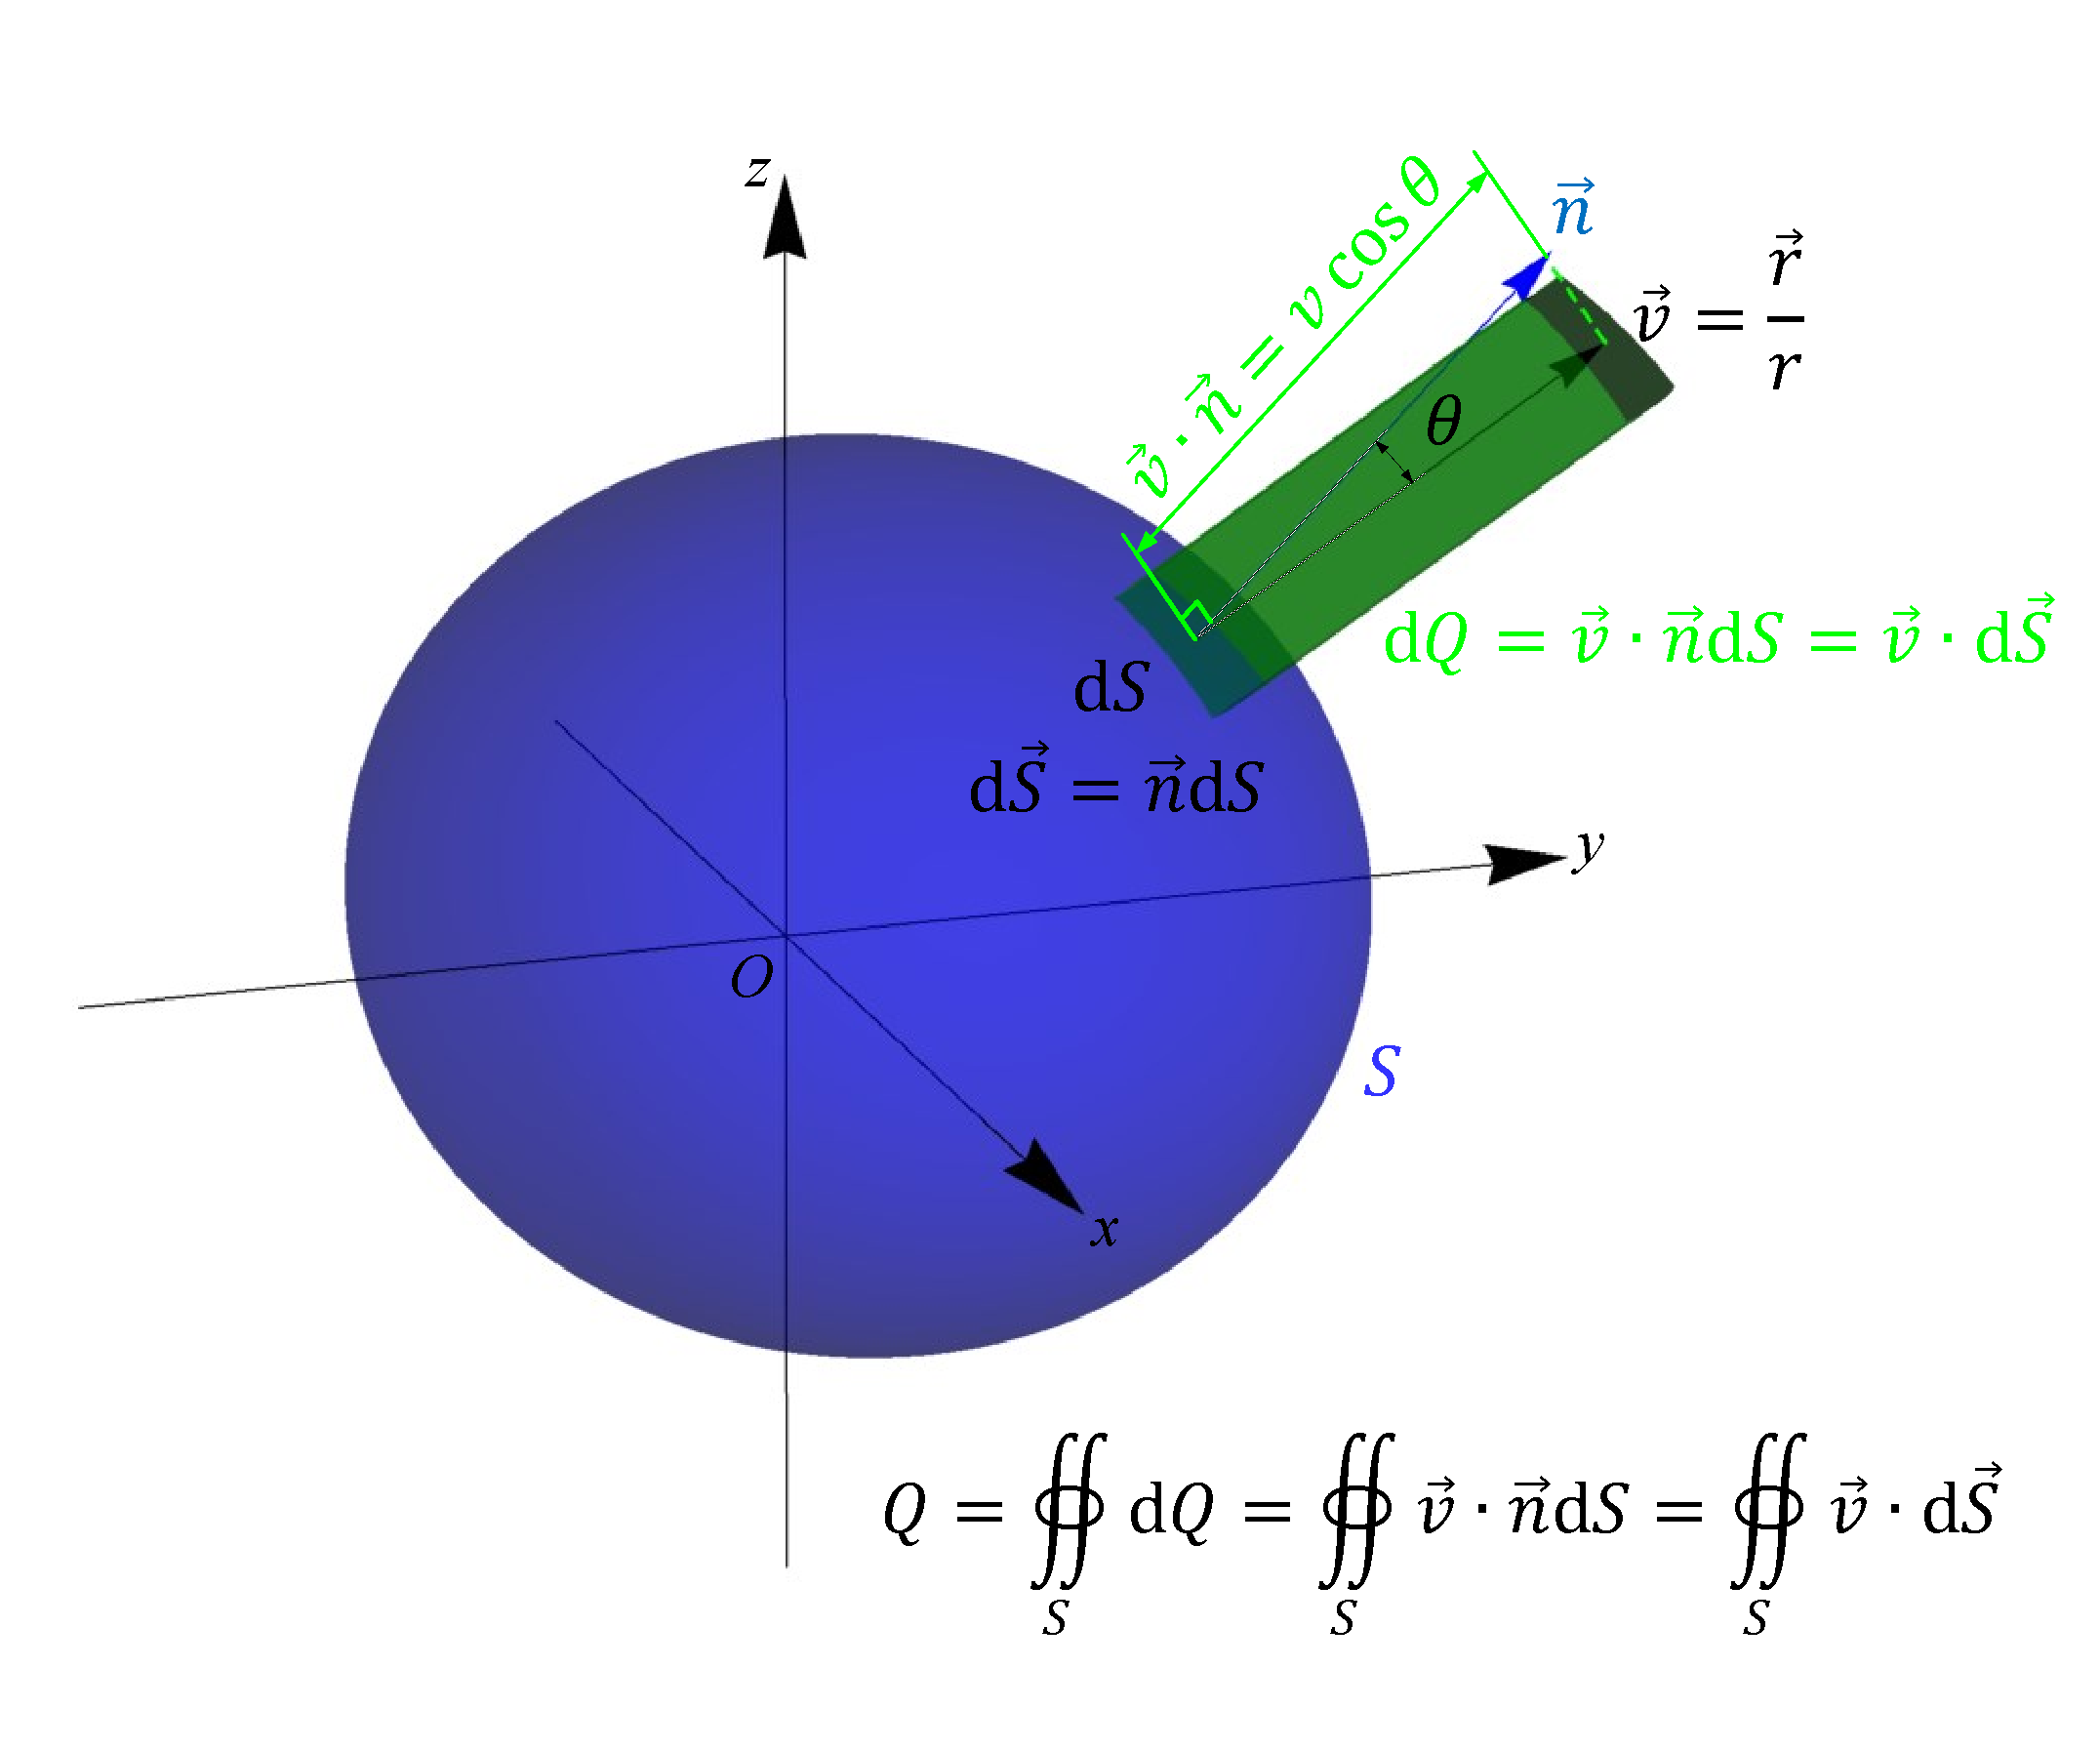
\includegraphics[height=0.58\textheight]{Figures25/Fig13-6-9-1.pdf} }}
\end{center}
\end{figure}
\addtocounter{figure}{-1}
\begin{figure}[H]
\addtocounter{figure}{1}
\begin{center}
\subfigure[]{\label{13-6-9-2} {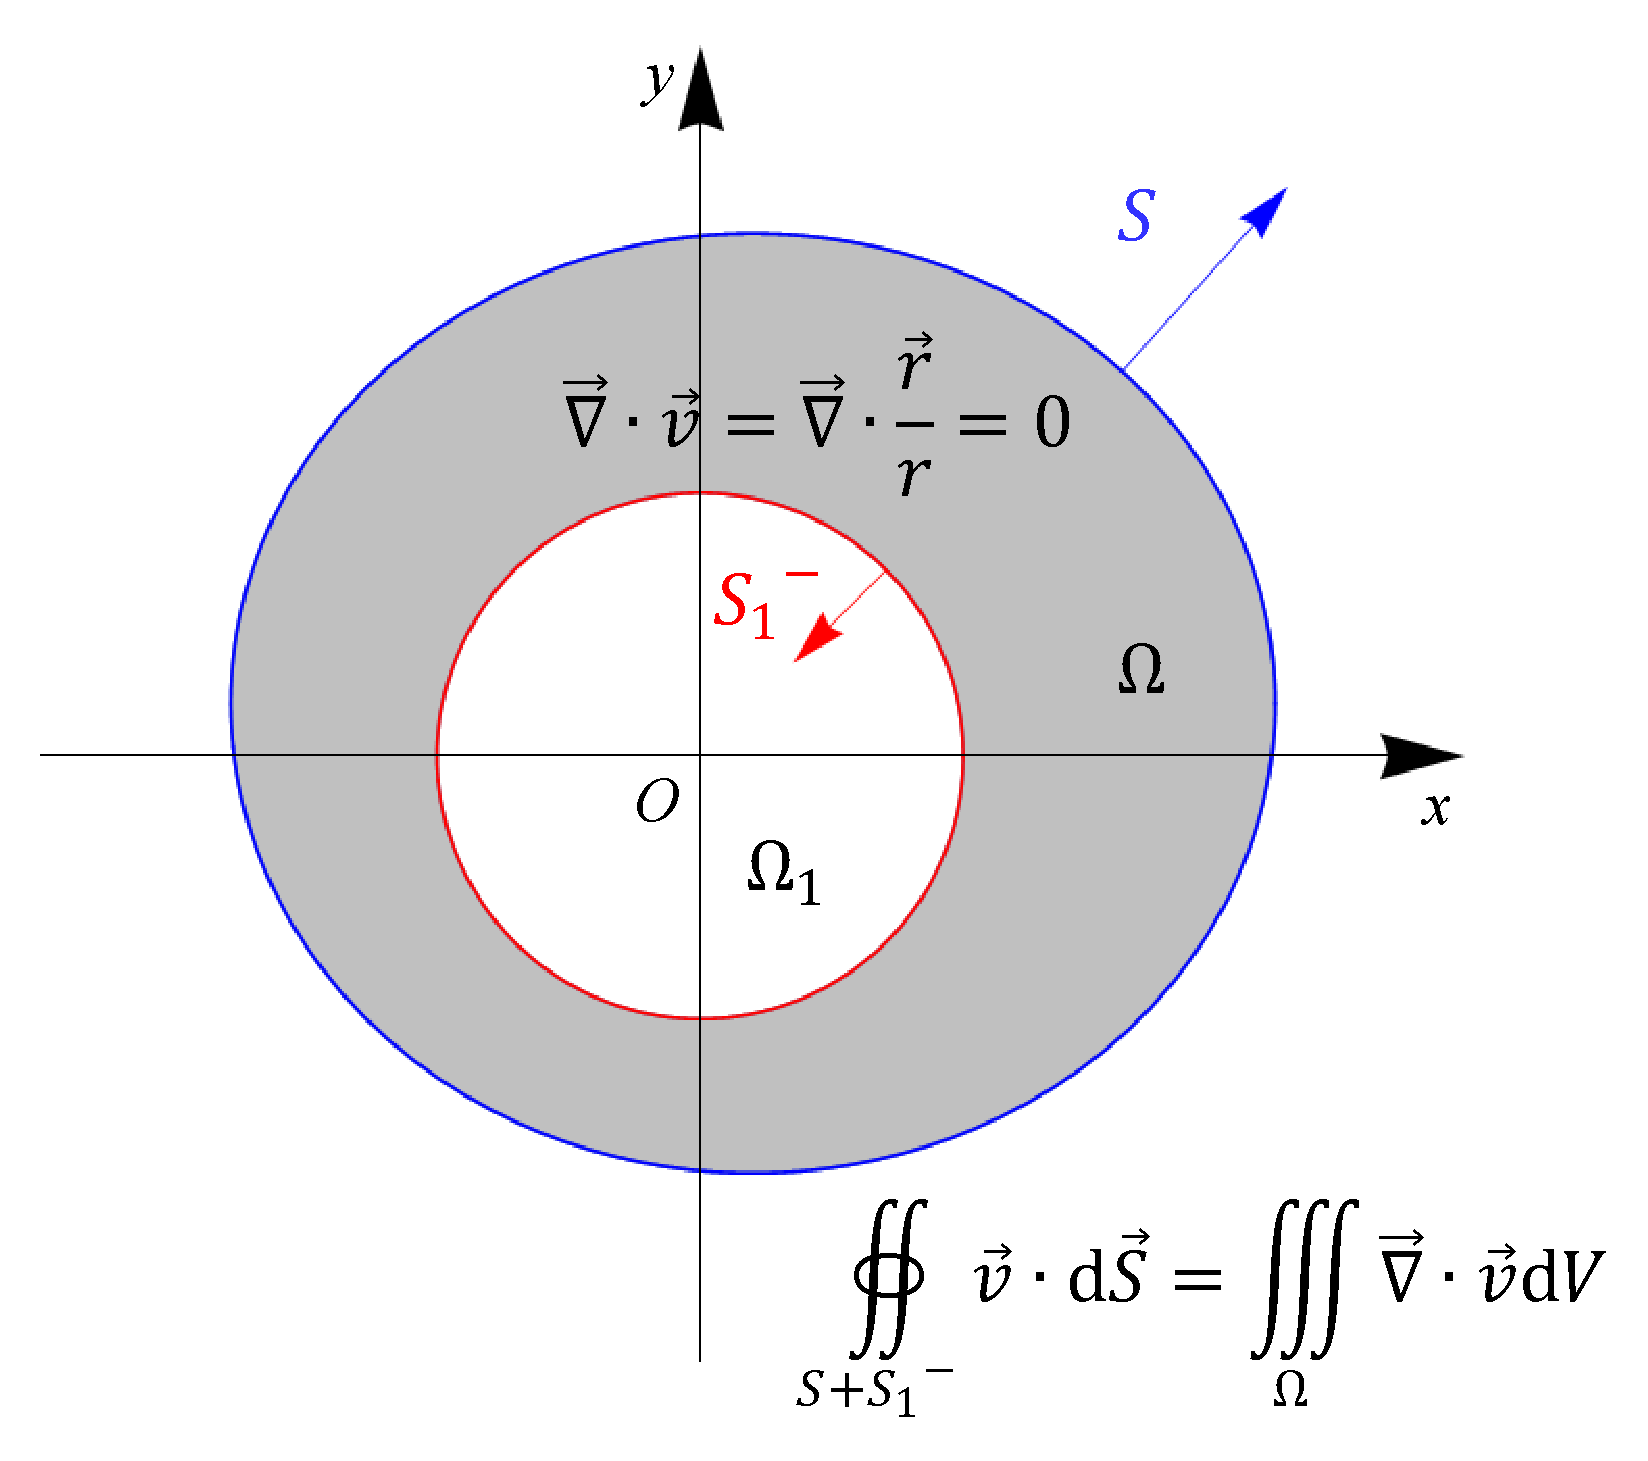
\includegraphics[height=0.6\textheight]{Figures25/Fig13-6-9-2.pdf} }}
\end{center}
\caption{习题13.6 9.题图示}
\label{13-6-9}
\end{figure}

\item证明下列向量场为无旋场:\\
(1)$\bm v=(x-x_0)\bm i+(y-y_0)\bm j+(z-z_0)\bm k$;\\
(2)$\bm v=yz(2x+y+z)\bm i+zx(x+2y+z)\bm j+xy(x+y+2z)\bm k$.

证明:(1)$\text{rot}\bm v=\bm\nabla\times\bm v=\begin{vmatrix}
\bm i&\bm j&\bm k\\
\ppx{}&\ppy{}&\ppz{}\\
x-x_0&y-y_0&z-z_0
\end{vmatrix}\\
=(\ppy{(z-z_0)}-\ppz{(y-y_0)},\ppz{(x-x_0)}-\ppx{(z-z_0)},\ppx{(y-y_0)}-\ppy{(x-x_0)})=(0,0,0)=\bm0$.

(2)$\bm v=(2xyz+y^2z+yz^2)\bm i+(zx^2+2xyz+xz^2)\bm j+(x^2y+xy^2+2xyz)\bm k$,
\[\begin{aligned}
\text{rot}\bm v&=\bm\nabla\times\bm v=\begin{vmatrix}
\bm i&\bm j&\bm k\\
\ppx{}&\ppy{}&\ppz{}\\
2xyz+y^2z+yz^2&zx^2+2xyz+xz^2&x^2y+xy^2+2xyz
\end{vmatrix}\\
&=(\ppy{(x^2y+xy^2+2xyz)}-\ppz{(zx^2+2xyz+xz^2)},\\
&\hspace{3cm}\ppz{(2xyz+y^2z+yz^2)}-\ppx{(x^2y+xy^2+2xyz)},\\
&\hspace{6cm}\ppx{(zx^2+2xyz+xz^2)}-\ppy{(2xyz+y^2z+yz^2)})\\
&=(x^2+2xy+2xz-(x^2+2xy+2zx),\\
&\hspace{3cm}2xy+y^2+2yz-(2xy+y^2+2yz),\\
&\hspace{6cm}2zx+2yz+z^2-(2zx+2yz+z^2))\\
&=\bm0.
\end{aligned}\]
\end{enumerate}
\subsection{习题13.1解答}
\begin{enumerate}
\item验证梯度算子$\bm\nabla$的下列性质,其中$\alpha,\beta$为任意常数,$f,g$为任意可微函数:\\
(1)$\bm\nabla(\alpha f+\beta g)=\alpha\bm\nabla+\beta\bm\nabla g$;\\
(2)$\bm\nabla(fg)=g\bm\nabla f+f\bm\nabla g$;\\
(3)$\bm\nabla(\frac fg)=\frac{g\bm\nabla f-f\bm\nabla g}{g^2}$(在$g$不等于零处成立).

证明:(1)\[\begin{split}
\bm\nabla(\alpha f+\beta g)&=(\pp{}x\bm i+\pp{}y\bm j+\pp{}z\bm k)(\alpha f+\beta g)\\
&=\pp{(\alpha f+\beta g)}x\bm i+\pp{(\alpha f+\beta g)}y\bm j+\pp{(\alpha f+\beta g)}z\bm k\\
&=(\alpha\pp fx+\beta\pp gx)\bm i+(\alpha\pp fy+\beta\pp gy)\bm j+(\alpha\pp fz+\beta\pp gz)\bm k\\
&=\alpha(\pp fx\bm i+\pp fy\bm j+\pp fz\bm k)+\beta(\pp gx\bm i+\pp gy\bm j+\pp gz\bm k)\\
&=\alpha\bm\nabla f+\beta\bm\nabla g.
\end{split}\]
(2)\[\begin{split}
\bm\nabla(fg)&=(\pp{}x\bm i+\pp{}y\bm j+\pp{}z\bm k)(fg)\\
&=\pp{(fg)}x\bm i+\pp{(fg)}y\bm j+\pp{(fg)}z\bm k\\
&=(g\pp fx+f\pp gx)\bm i+(g\pp fy+f\pp gy)\bm j+(g\pp fz+f\pp gz)\bm k\\
&=g(\pp fx\bm i+\pp fy\bm j+\pp fz\bm k)+f(\pp gx\bm i+\pp gy\bm j+\pp gz\bm k)\\
&=g\bm\nabla f+f\bm\nabla g.
\end{split}\]
(3)\[\begin{split}
\bm\nabla(\frac fg)&=(\pp{}x\bm i+\pp{}y\bm j+\pp{}z\bm k)(\frac fg)\\
&=\pp{}x(\frac fg)\bm i+\pp{}y(\frac fg)\bm j+\pp{}z(\frac fg)\bm k\\
&=\frac{g\pp fx-f\pp gx}{g^2}\bm i+\frac{g\pp fy-f\pp gy}{g^2}\bm j+\frac{g\pp fz-f\pp gz}{g^2}\bm k\\
&=\frac{g(\pp fx\bm i+\pp fy\bm j+\pp fz\bm k)-f(\pp gx\bm i+\pp gy\bm j+\pp gz\bm k)}{g^2}\\
&=\frac{g\bm\nabla f-f\bm\nabla g}{g^2}.
\end{split}\]
\item验证散度算子的下列性质(其中$f$为函数,$\bm u,\bm v$是向量场):
\[\bm\nabla\bm\cdot(\bm u\times\bm v)=-\bm u\bm\cdot\bm\nabla\times\bm v+\bm v\bm\cdot\bm\nabla\times\bm u.\]
证明:\[\begin{split}
\bm\nabla\bm\cdot(\bm u\times\bm v)&=(\pp{}x\bm i+\pp{}y\bm j+\pp{}z\bm k)\bm\cdot\begin{vmatrix}
\bm i&\bm j&\bm k\\
u_1(x,y,z)&u_2(x,y,z)&u_3(x,y,z)\\
v_1(x,y,z)&v_2(x,y,z)&v_3(x,y,z)
\end{vmatrix}\\
&=(\pp{}x\bm i+\pp{}y\bm j+\pp{}z\bm k)\bm\cdot[(u_2v_3-u_3v_2)\bm i+(u_3v_1-u_1v_3)\bm j+(u_1v_2-u_2v_2)\bm k]\\
&=\pp{(u_2v_3-u_3v_2)}x+\pp{(u_3v_1-u_1v_3)}y+\pp{(u_1v_2-u_2v_1)}z\\
&=\pp{u_2}xv_3+u_2\pp{v_3}x-\pp{u_3}xv_2-u_3\pp{v_2}x\\
&+\pp{u_3}yv_1+u_3\pp{v_1}y-\pp{u_1}yv_3-u_1\pp{v_3}y\\
&+\pp{u_1}zv_2+u_1\pp{v_2}z-\pp{u_2}zv_1-u_2\pp{v_1}z\\
&=u_1(\pp{v_2}z-\pp{v_3}y)+u_2(\pp{v_3}x-\pp{v_1}z)+u_3(\pp{v_1}y-\pp{v_2}x)\\
&+v_1(\pp{u_3}y-\pp{u_2}z)+v_2(\pp{u_1}z-\pp{u_3}x)+v_3(\pp{u_2}x-\pp{u_1}y)\\
&=-u_1(\pp{v_3}y-\pp{v_2}z)-u_2(\pp{v_1}z-\pp{v_3}x)-u_3(\pp{v_2}x-\pp{v_1}y)\\
&\quad+v_1(\pp{u_3}y-\pp{u_2}z)+v_2(\pp{u_1}z-\pp{u_3}x)+v_3(\pp{u_2}x-\pp{u_1}y)\\
&=-(u_1\bm i+u_2\bm j+u_3\bm k)\bm\cdot[(\pp{v_3}y-\pp{v_2}z)\bm i+(\pp{v_1}z-\pp{v_3}x)\bm j+(\pp{v_3}x-\pp{v_1}y)\bm k]\\
&\quad+(v_1\bm i+v_2\bm j+v_3\bm k)\bm\cdot[(\pp{u_3}y-\pp{u_2}z)\bm i+(\pp{u_1}z-\pp{u_3}x)\bm j+(\pp{u_2}x-\pp{u_1}y)\bm k]\\
&=-(u_1\bm i+u_2\bm j+u_3\bm k)\bm\cdot\begin{vmatrix}
\bm i&\bm j&\bm k\\
\pp{}x&\pp{}y&\pp{}z\\
v_1&v_2&v_3
\end{vmatrix}+(v_1\bm i+v_2\bm j+v_3\bm k)\bm\cdot\begin{vmatrix}
\bm i&\bm j&\bm k\\
\pp{}x&\pp{}y&\pp{}z\\
u_1&u_2&u_3
\end{vmatrix}\\
&=-\bm u\bm\cdot(\bm\nabla\times\bm v)+\bm v\bm\cdot(\bm\nabla\times\bm u)
\end{split}\]
%\[\begin{split}
%&-\bm u\bm\cdot(\bm\nabla\times\bm v)+\bm v\bm\cdot(\bm\nabla\times\bm u)\\
%=&-(u_1\bm i+u_2\bm j+u_3\bm k)\bm\cdot\begin{vmatrix}
%\bm i&\bm j&\bm k\\
%\pp{}x&\pp{}y&\pp{}z\\
%v_1&v_2&v_3
%\end{vmatrix}+(v_1\bm i+v_2\bm j+v_3\bm k)\bm\cdot\begin{vmatrix}
%\bm i&\bm j&\bm k\\
%\pp{}x&\pp{}y&\pp{}z\\
%u_1&u_2&u_3
%\end{vmatrix}\\
%=&-(u_1\bm i+u_2\bm j+u_3\bm k)\bm\cdot[(\pp{v_3}y-\pp{v_2}z)\bm i+(\pp{v_1}z-\pp{v_3}x)\bm j+(\pp{v_3}x-\pp{v_1}y)\bm k]\\
%&+(v_1\bm i+v_2\bm j+v_3\bm k)\bm\cdot[(\pp{u_3}y-\pp{u_2}z)\bm i+(\pp{u_1}z-\pp{u_3}x)\bm j+(\pp{u_2}x-\pp{u_1}y)\bm k]\\
%=&-u_1(\pp{v_3}y-\pp{v_2}z)-u_2(\pp{v_1}z-\pp{v_3}x)-u_3(\pp{v_3}x-\pp{v_1}y)\\
%&+v_1(\pp{u_3}y-\pp{u_2}z)+v_2(\pp{u_1}z-\pp{u_3}x)+v_3(\pp{u_2}x-\pp{u_1}y)
%\end{split}\]
\item设$\bm r=x\bm i+y\bm j+z\bm k,r=\sqrt{x^2+y^2+z^2}$:\\
(1)设$f(u)$为可微函数,求$\bm\nabla f(r)$;\\
(2)设$\bm F=f(r)\bm r$,求证$\bm\nabla\times\bm F\equiv\bm0$. 又问当$f$满足什么条件时,$\bm\nabla\bm\cdot\bm F=0$?

解:(1)\[\begin{split}
\bm\nabla f(r)&=\pp{f(r)}x\bm i+\pp{f(r)}y\bm j+\pp{f(r)}z\bm k\\
&=f'(r)\pp rx\bm i+f'(r)\pp ry\bm j+f'(r)\pp rz\bm k=f'(r)(\pp rx\bm i+\pp ry\bm j+\pp rz\bm k)\\
&=f'(r)(\frac x{\sqrt{x^2+y^2+z^2}}\bm i+\frac y{\sqrt{x^2+y^2+z^2}}\bm j+\frac z{\sqrt{x^2+y^2+z^2}}\bm k)\\
&=\frac{f'(r)}{\sqrt{x^2+y^2+z^2}}(x\bm i+y\bm j+z\bm k)=\frac{f'(r)}r\bm r.
\end{split}\]

(2)

i)证明:
\[\begin{split}
\bm\nabla\times\bm F&=\bm\nabla\times[f(r)\bm r]=\bm\nabla f(r)\times\bm r+f(r)\bm\nabla\times\bm r\\
&=\frac{f'(r)}r\bm r\times\bm r+f(r)\bm\nabla\times\bm r\\
&=0+f(r)\begin{vmatrix}
\bm i&\bm j&\bm k\\
\pp{}x&\pp{}y&\pp{}z\\
x&y&z
\end{vmatrix}\\
&=f(r)[(\pp zy-\pp yz)\bm i+(\pp xz-\pp zx)\bm j+(\pp yx-\pp xy)\bm k]\\
&=f(r)(0\bm i+0\bm j+0\bm k)=0.
\end{split}\]
ii)

$\because$
\[\begin{split}
\bm\nabla\bm\cdot\bm F&=\bm\nabla\bm\cdot[f(r)\bm r]=\bm\nabla f(r)\bm\cdot\bm r+f(r)\bm\nabla\bm\cdot\bm r=\frac{f'(r)}r\bm r\bm\cdot\bm r+f(r)(\pp xx+\pp yy+\pp zz)\\
&=\frac{\md f(r)}{\md r}r+3f(r)=0,
\end{split}\]
$\therefore$当$f(r)\neq0$时,$r\neq0$,
\[\frac{\md f(r)}{f(r)}=-3\frac{\md r}r,\]
$\therefore$
\[
\ln|f(r)|=-3\ln|r|+C_1,
\]
$\therefore$
\[
f(r)=\frac C{r^3},\text{$C$为任意常数}.
\]
\item验证旋度算子的下列基本公式:\\
(1)$\bm\nabla\times(\alpha\bm u+\beta\bm v)=\alpha\bm\nabla\times\bm u+\beta\bm\nabla\times\bm v$;\\
(2)$\bm\nabla\times(\bm\nabla f)=\bm0$;\\
(3)$\bm\nabla\bm\cdot(\bm\nabla\times\bm v)=0$.

证明:(1)\[\begin{split}
\bm\nabla\times(\alpha\bm u+\beta\bm v)&=\bm\nabla\times(\alpha u_1\bm i+\alpha u_2\bm j+\alpha u_3\bm k+\beta v_1\bm i+\beta v_2\bm j+\beta v_3\bm k)\\
&=\bm\nabla\times[(\alpha u_1+\beta v_1)\bm i+(\alpha u_2+\beta v_2)\bm j+(\alpha u_3+\beta v_3)\bm k]\\
&=\pp{(\alpha u_1+\beta v_1)}x+\pp{(\alpha u_2+\beta v_2)}y+\pp{(\alpha u_3+\beta v_3)}z\\
&=\alpha\pp{u_1}x+\beta\pp{v_1}x+\alpha\pp{u_2}y+\beta\pp{v_2}y+\alpha\pp{u_3}z+\beta\pp{v_3}z\\
&=\alpha(\pp{u_1}x+\pp{u_2}y+\pp{u_3}z)+\beta(\pp{v_1}x+\pp{v_2}y+\pp{v_3}z)\\
&=\alpha\bm\nabla\cdot\bm u+\beta\bm\nabla\cdot\bm v.
\end{split}\]
(2)当$f\in C^2$时
\[\begin{split}
\bm\nabla\times(\bm\nabla f)&=\bm\nabla\times(\pp fx\bm i+\pp fy\bm j+\pp fz\bm k)=\begin{vmatrix}
\bm i&\bm j&\bm k\\
\pp{}x&\pp{}y&\pp{}z\\
\pp fx&\pp fy&\pp fz
\end{vmatrix}\\
&=(\frac{\partial^2f}{\partial x\partial z}-\frac{\partial^2f}{\partial z\partial x})\bm i+(\frac{\partial^2f}{\partial z\partial x}-\frac{\partial^2f}{\partial x\partial z})\bm j+(\frac{\partial^2f}{\partial x\partial y}-\frac{\partial^2f}{\partial y\partial x})\bm k\\
&=0\bm i+0\bm j+0\bm k=\bm0.
\end{split}\]
(3)当$\bm v\in C^2$时
\[\begin{split}
\bm\nabla\bm\cdot(\bm\nabla\times\bm v)&=(\pp{}x\bm i+\pp{}y\bm j+\pp{}z\bm k)\bm\cdot\begin{vmatrix}
\bm i&\bm j&\bm k\\
\pp{}x&\pp{}y&\pp{}z\\
v_1(x,y,z)&v_2(x,y,z)&v_3(x,y,z)
\end{vmatrix}\\
&=(\pp{}x\bm i+\pp{}y\bm j+\pp{}z\bm k)\bm\cdot[(\pp{v_3}y-\pp{v_2}z)\bm i+(\pp{v_1}z-\pp{v_3}x)\bm j+(\pp{v_2}x-\pp{v_1}y)\bm k]\\
&=(\frac{\partial^2 v_3}{\partial x\partial y}-\frac{\partial^2 v_2}{\partial x\partial z})+(\frac{\partial^2 v_1}{\partial y\partial  z}-\frac{\partial^2 v_3}{\partial y\partial x})+(\frac{\partial^2 v_2}{\partial z\partial x}-\frac{\partial^2 v_1}{\partial z\partial y})\\
&=(\frac{\partial^2 v_3}{\partial x\partial y}-\frac{\partial^2 v_3}{\partial y\partial x})+(\frac{\partial^2 v_1}{\partial y\partial  z}-\frac{\partial^2 v_1}{\partial z\partial y})+(\frac{\partial^2 v_2}{\partial z\partial x}-\frac{\partial^2 v_2}{\partial x\partial z})\\
&=0.
\end{split}\]
\item求下列向量场的散度:\\
(1)$\bm v=xyz(x\bm i+y\bm j+z\bm k)$;\\
(2)$\bm v=(x\bm i+y\bm j+z\bm k)\times\bm c$;\\
(3)$\bm v=[(x\bm i+y\bm j+z\bm k)\bm\cdot\bm c](x\bm i+y\bm j+z\bm k)$(其中$\bm c$为常值向量).

解:(1)\[\begin{split}
\bm\nabla\bm\cdot\bm v&=\bm\nabla(xyz)\bm\cdot(x\bm i+y\bm j+z\bm k)+xyz\bm\nabla\bm\cdot(x\bm i+y\bm j+z\bm k)\\
&=(yz\bm i+xz\bm j+xy\bm k)\bm\cdot(x\bm i+y\bm j+z\bm k)+xyz(\pp xx+\pp yy+\pp zz)\\
&=xyz+xyz+xyz+3xyz=6xyz.
\end{split}\]
(2)\[\begin{split}
\bm\nabla\bm\cdot\bm v&=\bm c\bm\cdot[\bm\nabla\times(x\bm i+y\bm j+z\bm k)]-(x\bm i+y\bm j+z\bm k)\cdot(\bm\nabla\times\bm c)\\
&=\bm c\bm\cdot\begin{vmatrix}
\bm i&\bm j&\bm k\\
\pp{}x&\pp{}y&\pp{}z\\
x&y&z
\end{vmatrix}-(x\bm i+y\bm j+z\bm k)\bm\cdot\bm0\\
&=\bm c\bm\cdot[(\pp zy-\pp yz)\bm i+(\pp xz-\pp zx)\bm j+(\pp yx-\pp xy)\bm k]-0\\
&=\bm c\bm\cdot\bm0-0=0.
\end{split}\]
(3)记$\bm c=(c_1,c_2,c_3)$
\[\begin{split}
\bm\nabla\bm\cdot\bm v&=[(x\bm i+y\bm j+z\bm k)\bm\cdot\bm c]\bm\nabla\bm\cdot(x\bm i+y\bm j+z\bm k)+(x\bm i+y\bm j+z\bm k)\bm\cdot\bm\nabla[(x\bm i+y\bm j+z\bm k)\bm\cdot\bm c]\\
&=[(x\bm i+y\bm j+z\bm k)\bm\cdot\bm c](\pp xx+\pp yy+\pp zz)+(x\bm i+y\bm j+z\bm k)\bm\cdot\bm\nabla(c_1x+c_2y+c_3z)\\
&=3[(x\bm i+y\bm j+z\bm k)\bm\cdot\bm c]+(x\bm i+y\bm j+z\bm k)\bm\cdot(c_1\bm i+c_2\bm j+c_3\bm k)\\
&=3[(x\bm i+y\bm j+z\bm k)\bm\cdot\bm c]+(x\bm i+y\bm j+z\bm k)\bm\cdot\bm c\\
&=4(x\bm i+y\bm j+z\bm k)\bm\cdot\bm c.
\end{split}\]
\item求下列向量场的旋度:\\
(1)$\bm v=y^2z\bm i+z^2x\bm j+x^2y\bm k$;\\
(2)$\bm v=f(\sqrt{x^2+y^2+z^2})\bm c$(其中$\bm c$)为常值向量.

解:(1)\[\begin{split}
\bm\nabla\times\bm v=\begin{vmatrix}
\bm i&\bm j&\bm k\\
\pp{}x&\pp{}y&\pp{}z\\
y^2z&z^2x&x^2y
\end{vmatrix}=(x^2-2xz)\bm i+(y^2-2xy)\bm j+(z^2-2yz)\bm k.
\end{split}\]
(2)\[\begin{split}
\bm\nabla\times\bm v&=\bm\nabla\times[f(\sqrt{x^2+y^2+z^2})\bm c]\\
&=\bm\nabla f(\sqrt{x^2+y^2+z^2})\times\bm c+f(\sqrt{x^2+y^2+z^2})\bm\nabla\times\bm c\\
&=f'(\sqrt{x^2+y^2+z^2})(\frac x{\sqrt{x^2+y^2+z^2}}\bm i+\frac y{\sqrt{x^2+y^2+z^2}}\bm j+\frac z{\sqrt{x^2+y^2+z^2}}\bm k)\times\bm c+\bm0\\
&=\frac{f'(\sqrt{x^2+y^2+z^2})}{\sqrt{x^2+y^2+z^2}}(x\bm i+y\bm j+z\bm k)\times\bm c.
\end{split}\]
\end{enumerate}
\end{document}